%%%%%%%%%%%%%%%%%%%%%%%%%%%%%%%%%%%%%%%%%%%%%%%%%%%%%%%%%%%%%%%%%%%%%%%%%%%%%
%%% LaTeX-Rahmen fuer das Erstellen von Masterarbeiten
%%%%%%%%%%%%%%%%%%%%%%%%%%%%%%%%%%%%%%%%%%%%%%%%%%%%%%%%%%%%%%%%%%%%%%%%%%%%%

%%%%%%%%%%%%%%%%%%%%%%%%%%%%%%%%%%%%%%%%%%%%%%%%%%%%%%%%%%%%%%%%%%%%%%%%%%%%%
%%% allgemeine Einstellungen
%%%%%%%%%%%%%%%%%%%%%%%%%%%%%%%%%%%%%%%%%%%%%%%%%%%%%%%%%%%%%%%%%%%%%%%%%%%%%

\documentclass[12pt,a4paper]{report}
\usepackage[utf8]{inputenc}

\usepackage{amsmath}
\usepackage[scaled=0.92]{helvet}
\usepackage[scaled=1.1]{nimbusmononarrow}
\usepackage[T1]{fontenc}

\usepackage{eurosym}
\usepackage[english,ngerman]{babel}
\usepackage{bibgerm}
\usepackage{graphics, graphicx}
\usepackage[margin=10pt,font=small,labelfont=bf]{caption}
\usepackage{sistyle}
\usepackage{latexsym}
\usepackage{hyperref}
\usepackage[textwidth=14cm,textheight=22cm]{geometry}

%\footskip 2cm
\parskip 0.5ex plus 0.1ex minus 0.1ex
%\parindent0pt


% Kann nach persönlichem Geschmack verändert werden.
\usepackage{fancyhdr}
\pagestyle{fancy}
\fancyhead[LO,RE]{\textsl{\nouppercase{\leftmark}}}
\fancyhead[LE,RO]{\thepage}
\fancyfoot{}

%\fancyhead[LE,RO]{\textsl{\rightmark}}


% Kommentar-Style zum Einfügen von To-Do's Befehle: \todo , \note und \listoftodos
\usepackage[textsize=footnotesize,textwidth=0.8in]{todonotes} % Kommentare einschalten
%\usepackage[disable]{todonotes} % Kommentarausgabe ausschalten
\setlength{\marginparwidth}{0.8in} % Abstand vom Rand
\newcommand{\note}{\todo[inline,color=yellow,caption={}]} %Notiz über volle Seitenbreite


\begin{document}

%%%%%%%%%%%%%%%%%%%%%%%%%%%%%%%%%%%%%%%%%%%%%%%%%%%%%%%%%%%%%%%%%%%%%%%%%%%%
%%% hier steht die neue Titelseite
%%%%%%%%%%%%%%%%%%%%%%%%%%%%%%%%%%%%%%%%%%%%%%%%%%%%%%%%%%%%%%%%%%%%%%%%%%%%

\begin{titlepage}
 \begin{center}
  {\LARGE Eberhard Karls Universität Tübingen}\\
  {\large Mathematisch-Naturwissenschaftliche Fakultät\\
  Fachbereich Informatik\\[2cm]}
  {\Huge\bf  Titel\\[1.5cm]}
  {\Large Masterarbeit Informatik\\[3.5cm]}
  {\Large Vor- und Nachname}\\[0.5cm]
  Datum\\[4cm]
{\small\bf Betreuer}\\[0.5cm]
  \parbox{7cm}{\begin{center}{
  	\large Prof. Dr. Oliver Bringmann}\\
	  Lehrstuhl für Eingebettete Systeme\\
	  Fachbereich Informatik\\
	  Universität Tübingen
	  \end{center}}\hfill\parbox{7cm}{\begin{center}
  {\large Name Zweitgutachter}\\
	  Arbeitsbereich\\
	  Fachbereich Informatik\\
	  Universität Tübingen \end{center}
 }
  \end{center}
\end{titlepage}

%%%%%%%%%%%%%%%%%%%%%%%%%%%%%%%%%%%%%%%%%%%%%%%%%%%%%%%%%%%%%%%%%%%%%%%%%%%%
%%% Titelrückseite: Bibliographische Angaben
%%%%%%%%%%%%%%%%%%%%%%%%%%%%%%%%%%%%%%%%%%%%%%%%%%%%%%%%%%%%%%%%%%%%%%%%%%%%

\thispagestyle{empty}
\vspace*{\fill}
\begin{minipage}{11.2cm}
\textbf{Nachname, Vorname:}\\
\emph{Titel der Arbeit}\\ Masterarbeit Informatik\\
Eberhard Karls Universit"at T"ubingen\\
Bearbeitungszeitraum: von-bis
\end{minipage}
\newpage

%%%%%%%%%%%%%%%%%%%%%%%%%%%%%%%%%%%%%%%%%%%%%%%%%%%%%%%%%%%%%%%%%%%%%%%%%%%%

\pagenumbering{roman}
\setcounter{page}{1}

%%%%%%%%%%%%%%%%%%%%%%%%%%%%%%%%%%%%%%%%%%%%%%%%%%%%%%%%%%%%%%%%%%%%%%%%%%%%
%%% Seite I: Zusammenfassug, Danksagung
%%%%%%%%%%%%%%%%%%%%%%%%%%%%%%%%%%%%%%%%%%%%%%%%%%%%%%%%%%%%%%%%%%%%%%%%%%%%


\thispagestyle{plain}
\section*{Zusammenfassung}

Hier kommt die Zusammenfassung hin!!!
\newpage


\thispagestyle{plain}
\section*{Danksagung}

Hier kommen die Danksagungen hin (falls gewünscht)!!!

\newpage

%%%%%%%%%%%%%%%%%%%%%%%%%%%%%%%%%%%%%%%%%%%%%%%%%%%%%%%%%%%%%%%%%%%%%%%%%%%%%
%%% Erklaerung
%%%%%%%%%%%%%%%%%%%%%%%%%%%%%%%%%%%%%%%%%%%%%%%%%%%%%%%%%%%%%%%%%%%%%%%%%%%%%
\thispagestyle{empty}
\section*{Selbständigkeitserklärung}

%Hiermit versichere ich, dass ich die vorliegende Masterarbeit selbständig und nur mit den angegebenen Hilfsmitteln angefertigt habe und dass alle Stellen, die dem Wortlaut oder dem Sinne nach anderen Werken entnommen sind, durch Angaben von Quellen als Entlehnung kenntlich gemacht worden sind. Diese Masterarbeit wurde in gleicher oder ähnlicher Form in keinem anderen Studiengang als Prüfungsleistung vorgelegt.

% Erklärung aus dem Formular zur Anmeldung einer Bachelor-, Master- oder Diplomarbeit
% http://www.uni-tuebingen.de/fakultaeten/mathematisch-naturwissenschaftliche-fakultaet/fachbereiche/informatik/studium/downloads/allgemein-und-formulare.html
Hiermit erkläre ich, dass ich diese schriftliche Abschlussarbeit selbständig verfasst habe, keine anderen als die angegebenen Hilfsmittel und Quellen benutzt habe und alle wörtlich oder sinngemäß aus anderen Werken übernommenen Aussagen als solche gekennzeichnet habe.

\vskip 3cm

Ort, Datum	\hfill Unterschrift \hfill


%%%%%%%%%%%%%%%%%%%%%%%%%%%%%%%%%%%%%%%%%%%%%%%%%%%%%%%%%%%%%%%%%%%%%%%%%%%%%
%%% Inhaltsverzeichnis
%%%%%%%%%%%%%%%%%%%%%%%%%%%%%%%%%%%%%%%%%%%%%%%%%%%%%%%%%%%%%%%%%%%%%%%%%%%%%

\renewcommand{\baselinestretch}{1.3}
\small\normalsize

\tableofcontents

\renewcommand{\baselinestretch}{1}
\small\normalsize

\newpage

%%%%%%%%%%%%%%%%%%%%%%%%%%%%%%%%%%%%%%%%%%%%%%%%%%%%%%%%%%%%%%%%%%%%%%%%%%%%%
%%% Der Haupttext, ab hier mit arabischer Numerierung
%%% Mit \input{dateiname} werden die Datei `dateiname' eingebunden
%%%%%%%%%%%%%%%%%%%%%%%%%%%%%%%%%%%%%%%%%%%%%%%%%%%%%%%%%%%%%%%%%%%%%%%%%%%%%

\pagenumbering{arabic}
\setcounter{page}{1}

%% Introduction
%%%%%%%%%%%%%%%%%%%%%%%%%%%%%%%%%%%%%%%%%%%%%%%%%%%%%%%%%%%%%%%%%%%%
% Einleitung
%%%%%%%%%%%%%%%%%%%%%%%%%%%%%%%%%%%%%%%%%%%%%%%%%%%%%%%%%%%%%%%%%%%%

\chapter{Einleitung}\label{Einleitung}

Beginnen sollte die Arbeit mit einer kurzen Einführung und Motivation in das Themengebiet. Aus der Motivation lassen sich ggf. bestehende Probleme ableiten bzw. Probleme aufzeigen, die man in dieser Arbeit lösen möchte. Danach erfolgt die Beschreibung der Aufgabenstellung.

Die Arbeit gliedert sich dazu wie folgt: Die Grundlagen von BlaBlaBla 
werden in Kapitel \ref{Grundlagen} erarbeitet. 

\section*{Einige LaTeX-Hinweise}

Im folgenden wird das Einbinden einer Abbildung als `pdf-Datei' in ein
\LaTeX-Dokument gezeigt.

\begin{figure}[htb]
  \centering
  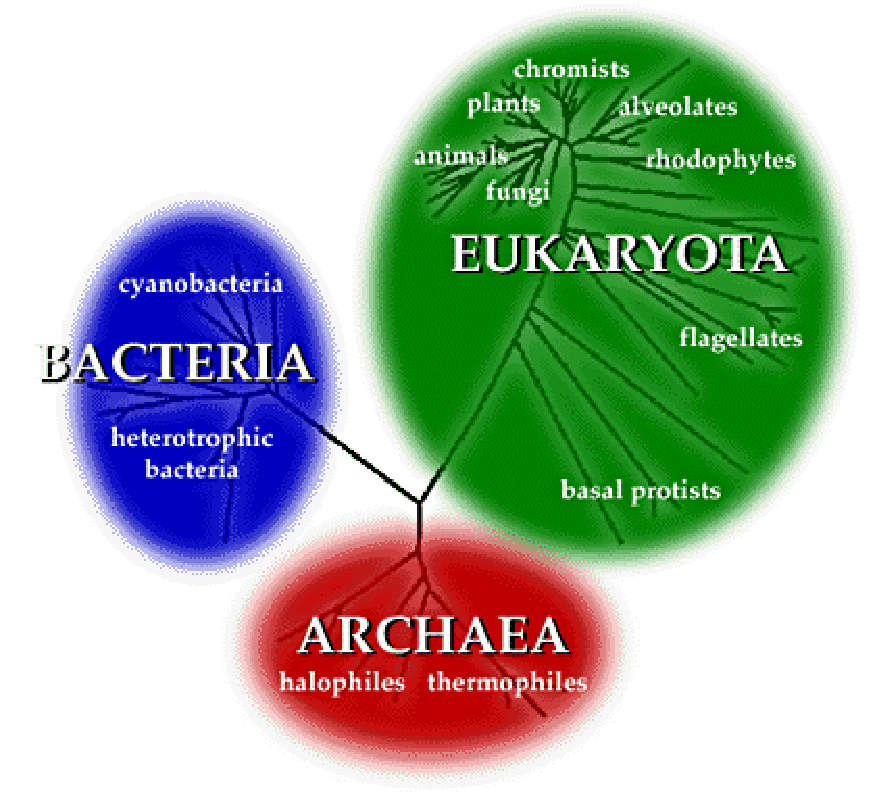
\includegraphics[width=0.5\textwidth]{figures/threedomains.pdf}
  \caption{Three Domains}
  \label{fig2_1}
\end{figure}

Abbildung \ref{fig2_1} zeigt ...

Tabellen können wie folgt erstellt werden:

\begin{table}[htb]
  \centering
  \begin{tabular}{|p{2.7cm}||l|c|r|}
    \hline
    \textbf{Spalte 1} 
    & \textbf{Spalte 2} 
    & \textbf{Spalte 3} 
    & \textbf{Spalte 4} \\
    \hline\hline
    xxx1111
    & xxxxxxx2222222
    & xxxxxx333333 
    & xxxxxxxxxx444444 \\
    \hline
    ...
    & ...
    & ...
    & ...\\
    \hline
  \end{tabular}
  \caption[Beispieltabelle mit langer Legende]{Beispieltabelle mit einer langen Legende, damit man sieht, dass in der Legende der Zeilenabstand verringert wurde. Außerdem soll auch der Font etwas kleiner gewählt werden. So sieht die ganze Umgebung kompakter aus.}
  \label{tabelle-1}
\end{table}


Eine Aufzählung geht wie folgt:
\begin{itemize}
	\item ...
	\item ...
\end{itemize}
Eine nummerierte Aufzählung:
\begin{enumerate}
	\item ...
	\item ...
\end{enumerate}

Betonungen sollen \emph{kursiv} gedruckt werden. 
\textbf{Fettdruck} ist auch möglich.

Referenzen: \cite{SaaSchTue97,TueConSaa96ismis,SchTueSaa98preprint}

\section[Arbeit]{Umfang der Arbeit}
,,Dies ist eine der meistgestellten Fragen. Natürlich verbirgt sich dahinter die Vermutung, die erzielbare Note sei – gutachterabhängig – mit der Seitenzahl korreliert (vgl. Abb.\ref*{fig2_2}). Nur
wie? Linear, normalverteilt, nach dem Gesetz vom abnehmenden Grenznutzen?
Tatsächlich kommt es auf die Qualität Ihrer Resultate an. Wenn Sie mit Ihrer Arbeit das Collatz-Problem, auch bekannt als Ulams Vermutung, widerlegen können, genügt eine Seite Inhalt mit dem Hinweis, die Zahl, welche die Vermutung widerlegt, befinde sich auf der beigefügten CD.

\begin{figure}[htb]
  \centering
  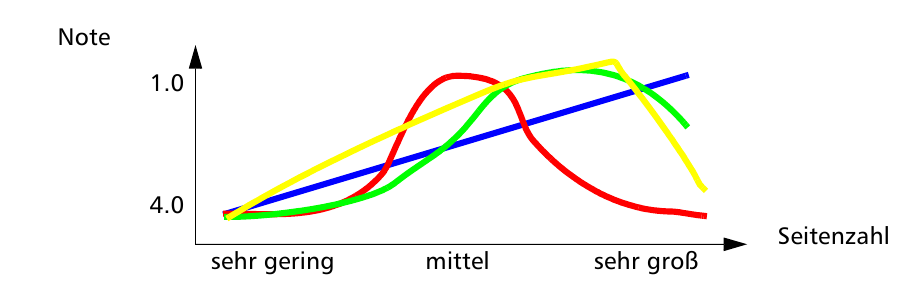
\includegraphics[width=0.9\textwidth]{figures/note-page.png}
  \caption[Verteilung: Seitenanzahl-Note]{Welcher Verteilung folgt die Note als Funktion der Seitenzahl? (aus \cite{Wegner16}) }
\label{fig2_2}
\end{figure}

Für alle, die nicht so viel Glück haben, soll die folgende Tabelle \ref{tabelle-2} auf Seite \pageref{tabelle-2} als Richtschnur
dienen. Dabei wurden Anhänge, Inhalts- und Abbildungsverzeichnisse sowie Stichwortverzeichnisse (sofern überhaupt vorhanden, da nicht üblich) nicht gerechnet.Bedenken Sie, dass Ihr Gutachter das alles gründlich lesen soll, der Zweitgutachter es vielleicht
auszugsweise lesen muss. Formulieren Sie deshalb knapp und auf den Punkt, vermeiden Sie Wiederholungen („Wir kommen nochmal auf das schwierige Problem der Softwareauswahl aus
Kapitel zwei zu sprechen, wo wir feststellten, dass ...“).
Längliche Passagen, etwa Programmstücke, Teile der Dokumentation, sehr lange Zitate (etwa ein Beweis, ein Gerichtsurteil, ein Zeitschriftenartikel im Wortlaut), Messreihen usw.
verbannen Sie in den Anhang (mit der Gewissheit, dass das kaum jemand gründlich lesen wird).
Aber auch bei den Anhängen ist weniger oft mehr. Noch umfangreichere Teile lassen sich auf
eine CD brennen, die der Arbeit beigefügt wird; allerdings ist umstritten, ob ein Gutachter sich
diese anschauen muss.

\begin{table}[tb]
  \centering
  \begin{tabular}{|c|c|c|c|} \hline
    \textbf{Art der Arbeit} & \textbf{Untergrenze} & \textbf{Obergrenze} & \textbf{Anmerkung} \\ \hline
		\hline
    Bachelor & 35 & 65 & ideal $\leq$ 50 \\ \hline
    Master & 50 & 85 & ideal $\leq$ 70 \\ \hline
  \end{tabular}
  \caption{Empfehlung zur Seitenanzahl der Arbeit}
  \label{tabelle-2}
\end{table}


Weil das Vorwort, der erste Abschnitt der Einleitung und die abschließende Zusammenfassung mit Ausblick immer gründlich gelesen werden, sollten Sie darauf besonderes Augenmerk
legen. In der Regel schreibt man die Einleitung und das Vorwort auch erst, wenn der restliche
Teil einschließlich Zusammenfassung (Fazit) steht, Spötter nennen das die Anpassung des
Anforderungsprofils an das tatsächlich erzielte Resultat.
Zuletzt ein Rat, wenn der Umfang der Arbeit erkennbar zu groß wird. So wie bei Seminarvorträgen Schnellersprechen das Problem eines zu umfangreichen Folienprogramms nicht
lösen kann, so wenig lässt sich mit typografischen Mitteln (kleinerem Font, engeren Zeilenabständen, breiteren Spalten) wesentlich Platz ohne Verlust an Lesbarkeit gewinnen. Sie kommen
nicht umhin, größere Teile der Arbeit zu streichen oder wesentlich zu straffen.
Dafür bieten sich oft die Kapitel an, in denen Sie den mühsamen Prozess der Lösungsfindung
einschließlich aller notwendigen Vorarbeiten und Diskussionen mit dem Anwender dokumentiert haben. Hinter solchen längeren Beschreibungen steckt der verständliche Wunsch, der Gutachter möge honorieren, dass Sie unglaublich mit dem Auftraggeber, der undurchsichtigen
Software, dem abstürzenden Computer u.a.m. kämpfen mussten und vieles zunächst nicht so
funktionierte, wie gedacht.
Leser sind aber wie Restaurantgäste, Gutachter ähneln Gourmetkritikern. Sie sind mitleidslos und schauen nur auf den Teller vor sich. Sie wollen nichts davon wissen, dass frische Seezunge heute enorm schwierig zu beschaffen war und der Jungkoch sich am Gratin die Finger
verbrannt hat. Halten Sie Ihre Schwierigkeiten in einem ehrlich geschriebenen 10-Zeilen-Abschnitt der Zusammenfassung fest, als Teil der Selbstreflektion, die immer zu einer
Abschlussarbeit gehört, und streichen Sie schweren Herzens Teile der Entwicklungssaga.'' (aus \cite{Wegner_engl16})


\newpage

%%
%%%%%%%%%%%%%%%%%%%%%%%%%%%%%%%%%%%%%%%%%%%%%%%%%%%%%%%%%%%%%%%%%%%%
% Grundlagen
%%%%%%%%%%%%%%%%%%%%%%%%%%%%%%%%%%%%%%%%%%%%%%%%%%%%%%%%%%%%%%%%%%%%

\chapter{Grundlagen}
  \label{Grundlagen}

Ziel dieses Kapitels ist eine Einführung in die Thematik BlaBlaBla ...

\section{Abschnittsüberschrift}
  \label{Abschnittslabel} 

BlaBlaBla ...

\subsection{Unterabschnittsüberschrift}
  \label{Unterabschnittslabel}

BlaBlaBla ...


Bevor wir uns der Auswertung bzw. Bewertung der gewonnenen Primärdaten zuwenden, wollen wir zunächst einige grundlegende Begriffe der deskriptiven Statistik wiederholen.
\section{Stichproben}

Grundsätzlich haben wir es bei Microarrayexpressionsdaten mit einer {\em Stichprobe} aus einer {\em Population (Grundgesamtheit)} zu tun.   
Wir bezeichnen nun im allgemeinen mit $X=\{x_1,x_2,\ldots,x_n\}$ die Beobachtungsdaten vom Umfang $n$. 
Diese Daten sollen mit statistischen Kenngrößen beschrieben werden. Aus diesen will man möglichst zuverlässig auf die zugrundeliegende Verteilung in der Grundgesamtheit schließen. Hierzu verwenden wir die {\bf Lage-} und {\bf Streuparameter}. Zunächst wenden wir uns aber der Häufigkeits- und Summenhäufigkeitsverteilung zu, die sowohl graphisch als auch numerisch einen Eindruck über die Verteilung von $X$ bieten. Dafür betrachten wir diskrete Verteilungen.

Gegeben sei eine Stichprobe $(X_1,X_2,\ldots,X_n)$. Eine Funktion $Z_n=Z(X_1,\ldots,X_n)$ wird als {\em Stichprobenfunktion} bezeichnet. Sie ist selber eine Zufallsgröße.

\subsection{Häufigkeiten und Histogramm}
In der Stichprobe $X$ trete der Wert $x_i$ genau $n_i$ mal auf, $i=1,2,\ldots m$. Dann ist $\sum_i n_i = n$. Der Quotient $n_i/n$ ist die {\em relative Häufigkeit} für das Eintreten des Ereignisses ``$X=x_i$''.
Die Menge der relativen Häufigkeiten $\{n_1/n,n_2/n,\ldots, n_m/n\}$ heißt {\em Häufigkeitsverteilung} von $X$. Ferner heißt die Menge $\{s_1,\ldots,s_m\}$ mit $s_i=\sum_{k=1}^{i}n_k/n$ die {\em Summenhäufigkeitsverteilung} von $X$.

Für die graphische Darstellung der Häufigkeitsverteilung wird das {\em Histogramm} gewählt. für die Summenhäufigkeitsverteilung die {\em Treppenfunktion}.

Wenn wir natürlich Zahlen mit Komma haben, so sieht das in Deutsch irgendwie seltsam aus, z.B. $0,7$. Ich nehme dafür den SIstyle: $\SI{0,7}{}$ usf.  Oder nett ist auch: \SI{9.3e5}{km}

\todo{Mit diesem Kommando kann man eigene Kommentare am Spaltenrand hinzufügen.}
\note{Mit diesem Kommando kann man eigene Kommentare in der Textspalte hinzufügen.}

%
\subsection{Wichtige Verteilungen}

\subsubsection{Die Normalverteilung}
Die Dichte der Normalverteilung ist gegeben durch
\begin{equation}\label{dichtenormal}
g(x) = \frac{1}{2\pi\sigma}\cdot e^{-\frac{(x-\mu)^2}{2\sigma^2}}
\end{equation}
wobei $\mu$ (Lage) der Mittelwert und $\sigma$ (Breite) die Standardabweichung der Normalverteilung ist. 
Durch die $z$-Transformation lässt sich die Normalverteilung auf die Standardnormalverteilung mit $\mu=0$ und $\sigma=1$ transformieren.

Die Normalverteilung bildet die Basis fast der gesamten statistischen Theorie. \footnote{ 
	\glqq Everyone believes in the normal law, the experimenters because they imagine it is a mathematical theorem, and the mathematicians because they think it is an experimental fact.\grqq{} (Gabriel Lippman, in Poincar's Calcul de probabilité, 1896)}. Auch bei der Analyse der Microarraydaten werden wir sehr oft von der Annahme der Normalverteilung Gebrauch machen. Allerdings sollten wir uns klarmachen, dass  rein experimentell zahlreiche Untersuchungen gezeigt haben, dass die echten Fehler selten, wenn überhaupt normal verteilt sind.


\section{Schätzung von Parametern}
Allgemein erhofft man sich beim Ziehen einer Stichprobe, einen unbekannten Parameter $\gamma$ der Grundgesamtheit, z.B. den Mittelwert, aus der Stichprobe zu schätzen.
\subsection{Eigenschaften von Punktschätzungen}

\newpage

%%
%%%%%%%%%%%%%%%%%%%%%%%%%%%%%%%%%%%%%%%%%%%%%%%%%%%%%%%%%%%%%%%%%%%%
% Diskussion und Ausblick
%%%%%%%%%%%%%%%%%%%%%%%%%%%%%%%%%%%%%%%%%%%%%%%%%%%%%%%%%%%%%%%%%%%%

\chapter{Stand der Technik}
  \label{SOTA}
Während im Grundlagenkapitel notwendige Begrifflichkeiten, Datenstrukturen, Basisalgorithmen oder Hardware-Architekturen vorgestellt werden, befasst sich dieser Abschnitt mit einer kurzen Diskussion existierender Ansätze und deren Probleme.

Je nach Themenstellung kann dieser Abschnitt auch entfallen. Eine kurze Diskussion kann in diesem Fall entweder in der Aufgabenstellung (Kapitel \ref{Grundlagen}) oder zu Beginn des eigenen Konzepts (Kapitel \ref{Konzept}) erfolgen. 

\newpage

%%
%%%%%%%%%%%%%%%%%%%%%%%%%%%%%%%%%%%%%%%%%%%%%%%%%%%%%%%%%%%%%%%%%%%%
% Diskussion und Ausblick
%%%%%%%%%%%%%%%%%%%%%%%%%%%%%%%%%%%%%%%%%%%%%%%%%%%%%%%%%%%%%%%%%%%%

\chapter{Konzept}
  \label{Konzept}

Mit das Wichtigste natürlich!

Hier wird der eigene Ansatz vorgestellt. Der Titel sollte natürlich nicht einfach Konzept heißen, sondern konkret den eigenen Ansatz benennen.


\newpage

%%
%%%%%%%%%%%%%%%%%%%%%%%%%%%%%%%%%%%%%%%%%%%%%%%%%%%%%%%%%%%%%%%%%%%%
% Diskussion und Ausblick
%%%%%%%%%%%%%%%%%%%%%%%%%%%%%%%%%%%%%%%%%%%%%%%%%%%%%%%%%%%%%%%%%%%%

\chapter{Ergebnisse}
  \label{Ergebnisse}

Hier sollen die erreichten Ergebnisse vorgestellt werden. Hierzu zählt die Vorstellung des Versuchsaufbaus sowie die geeignete Aufbereitung und Diskussion der Ergebnisse. Mehrwert oder Nutzen benennen!

\newpage

%%
%%%%%%%%%%%%%%%%%%%%%%%%%%%%%%%%%%%%%%%%%%%%%%%%%%%%%%%%%%%%%%%%%%%%
% Diskussion und Ausblick
%%%%%%%%%%%%%%%%%%%%%%%%%%%%%%%%%%%%%%%%%%%%%%%%%%%%%%%%%%%%%%%%%%%%

\chapter{Zusammenfassung und Ausblick}
  \label{Zusammenfassung}

Zusammenfassung der Arbeit unter Verwendung der eingeführten Begrifflichkeiten. Hier darf davon ausgegangen werden, dass der Leser die Arbeit gelesen hat bzw. kennt. Ferner sollte ein Ausblick auf Erweiterungsmöglichkeiten oder sich ergebende Forschungsfragen gegeben werden.

\newpage

%%%%%%%%%%%%%%%%%%%%%%%%%%%%%%%%%%%%%%%%%%%%%%%%%%%%%%%%%%%%%%%%%%%%%%%%%%%%%
%%% Bibliographie
%%%%%%%%%%%%%%%%%%%%%%%%%%%%%%%%%%%%%%%%%%%%%%%%%%%%%%%%%%%%%%%%%%%%%%%%%%%%%

\addcontentsline{toc}{chapter}{Literaturverzeichnis}

\bibliographystyle{alpha}
\bibliography{mylit}
%% Obige Anweisung legt fest, dass BibTeX-Datei `mylit.bib' verwendet
%% wird. Hier koennen mehrere Dateinamen mit Kommata getrennt aufgelistet
%% werden.

\newpage
\appendix
%%%%%%%%%%%%%%%%%%%%%%%%%%%%%%%%%%%%%%%%%%%%%%%%%%%%%%%%%%%%%%%%%%%%%%%%%%%%%
%%% Abk"urzungsverzeichnis
%%%%%%%%%%%%%%%%%%%%%%%%%%%%%%%%%%%%%%%%%%%%%%%%%%%%%%%%%%%%%%%%%%%%%%%%%%%%%

\addcontentsline{toc}{chapter}{Abk"urzungsverzeichnis}
\chapter*{Abk"urzungsverzeichnis\markboth{ABKÜRZUNGSVERZEICHNIS}{ABKÜRZUNGSVERZEICHNIS}}

\begin{tabbing}
	\textbf{FACTOTUM}\hspace{1cm}\=Schrott\kill
	\textbf{DFG}\>Datenflussgraph \\
	\textbf{...} \> ...\\
\end{tabbing}

\newpage

%%%%%%%%%%%%%%%%%%%%%%%%%%%%%%%%%%%%%%%%%%%%%%%%%%%%%%%%%%%%%%%%%%%%%%%%%%%%%
%%% Abbildungsverzeichnis
%%%%%%%%%%%%%%%%%%%%%%%%%%%%%%%%%%%%%%%%%%%%%%%%%%%%%%%%%%%%%%%%%%%%%%%%%%%%%

\renewcommand{\baselinestretch}{1.3}
\small\normalsize

\addcontentsline{toc}{chapter}{Abbildungsverzeichnis}
\listoffigures

\renewcommand{\baselinestretch}{1}
\small\normalsize

\newpage

%%%%%%%%%%%%%%%%%%%%%%%%%%%%%%%%%%%%%%%%%%%%%%%%%%%%%%%%%%%%%%%%%%%%%%%%%%%%%
%%% Tabellenverzeichnis
%%%%%%%%%%%%%%%%%%%%%%%%%%%%%%%%%%%%%%%%%%%%%%%%%%%%%%%%%%%%%%%%%%%%%%%%%%%%%

\renewcommand{\baselinestretch}{1.3}
\small\normalsize

\addcontentsline{toc}{chapter}{Tabellenverzeichnis}
\listoftables

\renewcommand{\baselinestretch}{1}
\small\normalsize

\newpage

%%%%%%%%%%%%%%%%%%%%%%%%%%%%%%%%%%%%%%%%%%%%%%%%%%%%%%%%%%%%%%%%%%%%%%%%%%%%%
%%% Ende
%%%%%%%%%%%%%%%%%%%%%%%%%%%%%%%%%%%%%%%%%%%%%%%%%%%%%%%%%%%%%%%%%%%%%%%%%%%%%

\end{document}
